\documentclass[lang=cn,10pt]{elegantbook}

\title{计算机图形学基础}
\subtitle{第五版 \  中文译本}

\author{Steve Marschner \& Peter Shirley}
\institute{Cornell University \& NVIDIA}
\date{February 2021}
\version{Fifth edition}
\bioinfo{译者}{buding}

\extrainfo{Stay hungry. Stay foolish. —— Steve Jobs}

\setcounter{tocdepth}{3}

\logo{logo.png}
\cover{cover.png}

% 本文档命令
\usepackage{array}
\usepackage{xcolor}
\definecolor{lightgreen}{RGB}{99,140,94}
\newcommand{\ccr}[1]{\makecell{{\color{#1}\rule{1cm}{1cm}}}}

% 修改标题页的橙色带
% \definecolor{customcolor}{RGB}{32,178,170}
% \colorlet{coverlinecolor}{customcolor}

\begin{document}

\maketitle

\frontmatter

\chapter{前言}

本版本的《计算机图形学基础》包括对阴影着色、光线反射和路径追踪等材料的大量重写,以及对全书的许多校正。本书对基于物理的材料和基于物理的渲染等技术进行了更好的介绍,这些技术在实际应用中逐渐占据主导地位。现在这些材料得到更好的整合,我们认为这本书很好地匹配了目前许多教师组织图形课程的方式。  

本书的组织结构与第四版基本相似。在多年来对本书进行修订的过程中,我们努力保留了早期版本中非正式的、直观的表述风格,同时也提高了本书的一致性、准确性和完整性。我们希望读者会发现,这本书是一个吸引人的平台,适合于各种计算机图形学课程。

\section{关于封面}

封面图片来自 J.W.Baker 的《水中之虎》(画布上的拉丝和喷枪亚克力,16英寸x20英寸),www.jwbart.com。  

老虎的主题是指 Alain Fournier(1943-2000)1998年在康奈尔大学的一次研讨会上的精彩演讲。他的演讲是对老虎动作进行的令人回味的口头描述。他总结了自己的观点:  

尽管在过去的35年里,计算机图形学的建模和渲染已经有了巨大的进展,但我们仍然无法自动模拟在河中游泳的老虎的所有精彩细节。我所说的自动是指不需要艺术家或专家进行仔细的手动调整的方式。    

坏消息是,我们还有很长的路没走。  

好消息是,我们还有很长的路要走。

\section{线上资源}

本书的网址是 http://www.cs.cornell.edu/\~{}srm/fcg5/ 。我们将继续维护本书的勘误表和课程链接,以及与本书风格相符的教学材料。本书中的大多数图片都是 Adobe Illustrator 格式的,我们很乐意根据需要将特定图片转换为可移植格式。请随时通过 srm@cs.cornell.edu 或 ptrshrl@gmail.com 与我们联系。  

\chapter{致谢}

以下人士提供了对于本书各版本的有用信息、评论或者反馈:Ahmet O˘guz Aky¨uz, Josh Andersen, Beatriz Trinch˜ao Andrade Zeferino Andrade, Bagossy Attila, Kavita Bala, Mick Beaver, Robert Belleman, Adam Berger, Adeel Bhutta, Solomon Boulos, Stephen Chenney, Michael Coblenz, Greg Coombe, Frederic Cremer, Brian Curtin, Dave Edwards, Jonathon Evans, Karen Feinauer, Claude Fuhrer, Yotam Gingold, Amy Gooch, Eungyoung Han, Chuck Hansen, Andy Hanson, Razen Al Harbi, Dave Hart, John Hart, Yong Huang, John “Spike” Hughes, Helen Hu, Vicki Interrante, Wenzel Jakob, Doug James, Henrik Wann Jensen, Shi Jin, Mark Johnson, Ray Jones, Revant Kapoor, Kristin Kerr, Erum Arif Khan, Mark Kilgard, Fangjun Kuang, Dylan Lacewell, Mathias Lang, Philippe Laval, Joshua Levine, Marc Levoy, Howard Lo, Joann Luu, Mauricio Maurer, Andrew Medlin, Ron Metoyer, Keith Morley, Eric Mortensen, Koji Nakamaru, Micah Neilson, Blake Nelson, Michael Nikelsky, James O’Brien, Hongshu Pan , Steve Parker, Sumanta Pattanaik, Matt Pharr, Ken Phillis Jr, Nicol`o Pinciroli, Peter Poulos, Shaun Ramsey, Rich Riesenfeld, Nate Robins, Nan Schaller, Chris Schryvers, Tom Sederberg, Richard Sharp, Sarah Shirley, Peter-Pike Sloan, Hannah Story, Tony Tahbaz, JanPhillip Tiesel, Bruce Walter, Alex Williams, Amy Williams, Chris Wyman, Kate Zebrose, and Angela Zhang。  

Ching-Kuang Shene 和 David Solomon 允许我们借用他们的例子。 Henrik Wann Jensen、Eric Levin、Matt Pharr 和 Jason Waltman 慷慨地提供了图片。 Brandon Mansfield 帮助改进了关于光线追踪的分层包围体的探讨。 Philip Greenspun (philip.greenspun.com) 热心地允许我们使用他的照片。 John “Spike” Hughes 帮助改进了对抽样理论的探讨。 Wenzel Jakob 的 Mitsuba 渲染器在创建许多图形方面非常宝贵。我们非常感谢 J.W. Baker 帮助创作了 Pete 设想的封面。他除了是一位才华横溢的艺术家之外,也是一位非常愉快的工作伙伴。  

本书的章节注释中引用了许对编写本书有帮助的著作。然而,有几本影响了本书内容和表现形式的关键文献值得在此特别表彰。其中包括两本经典的计算机图形学教材,我们都是从这两本教材中学习的基础知识——《计算机图形学:原理与实践》(Foley、Van Dam、Feiner 和 Hughes,1990 年)和《计算机图形学》(Hearn 和 Baker,1986 年)。其他文本包括 Alan Watt 的两本有影响力的书籍 (Watt, 1993, 1991), Hill的《使用OpenGL的计算机图形》(Francis S. Hill, 2000), Angel的《交互式计算机图形学:使用 OpenGL 的自上而下方法》(Angel, 2002), Hugues Hoppe 的华盛顿大学论文 (Hoppe, 1994) 和 Rogers 的两篇优秀的图形学文章 (D. F. Rogers, 1985, 1989)。  

我们要特别感谢 Alice 和 Klaus Peters 鼓励 Pete 撰写本书的第一版,感谢他们在帮助完成本书方面的伟大才能。他们对作者的耐心以及竭尽所能奉献于使本书成为最好的书籍对本书的出版起了重要的作用。如果没有他们的非凡努力,这本书肯定不会存在。 

\rightline{Steve Marschner,伊萨卡,纽约}

\rightline{Peter Shirley,盐湖城,犹他州}

\rightline{2021年2月}

\chapter{作者}

Steve Marschner是康奈尔大学的计算机科学教授。他于1993年在布朗大学获得理学学士学位,1998年在康奈尔大学获得博士学位。在2002年加入康奈尔大学之前,他在微软研究院和斯坦福大学担任研究职务。他是2015年SIGGRAPH计算机图形学成就奖的获得者和2003年技术学院奖的共同获得者。

Peter Shirley是英伟达公司的杰出研究科学家。他曾在印第安纳大学、康奈尔大学和犹他大学担任学术职务。他于1985年获得里德学院的物理学学士学位,1991年获得伊利诺伊大学的计算机科学博士学位。

\tableofcontents

\mainmatter

\chapter{图形学介绍}

计算机图形学这个术语描述了任何使用计算机来创建和操作图像的情况。本书介绍了可用于创建各种图像的算法和数学工具——逼真的视觉效果、丰富的技术插图或精美的计算机动画。图形可以是二维的,也可以是三维的;图像可以是完全合成的,也可以是通过处理照片产生的。本书是关于基本算法和数学的,特别是那些用于制作三维物体和场景的合成图像的算法。

实际上,做计算机图形不可避免地需要了解特定的硬件、文件格式,通常还需要一个或两个图形API(参见1.3节)。计算机图形学是一个快速发展的领域,因此这些知识的具体内容是在不断更新变化。因此,在本书中,我们尽力避免依赖任何特定的硬件或API。我们鼓励读者用他们的软件和硬件环境的相关文档来补充此文本。幸运的是,计算机图形文化有足够的标准术语和概念,本书的讨论应能很好地反映到大多数环境。


\remark{ API:应用程序编程接口}  

本章定义了一些基本术语,并提供了一些历史背景,以及与计算机图形相关的信息来源。

\section{图形学领域}

对任何领域强加分类都是危险的,但大多数图形从业者会对计算机图形的以下主要领域达成一致:

\begin{itemize}
\item 建模涉及的是形状和外观属性的数学规范化,这种方式可以存储在计算机上。例如,可以将咖啡杯描述为一组有序的三维点,以及一些连接这些点的插值规则和一个描述光线如何与杯子作用的反射模型。
\item 渲染是一个从艺术中继承下来的术语,涉及到从三维计算机模型创建阴影图像。
\item 动画是一种通过图像序列创造运动幻觉的技术。动画使用建模和渲染,但增加了随着时间移动的关键问题,这在基本的建模和渲染中通常无法处理。
\end{itemize}

还有许多其他涉及计算机图形的领域,关于它们是否属于图形学的核心领域,仁者见仁,智者见智。这些内容在本书都至少有所提及。此类相关领域包括以下内容:
\begin{itemize}
\item 用户接口涉及输入设备,例如鼠标和平板电脑、应用程序、图像对用户的反馈以及其他感官反馈的接口。从历史上看,该领域与图形有关,主要是因为计算机图形的研究人员最早接触到了现在无处不在的输入和输出设备。
\item 虚拟现实试图让用户沉浸在一个三维虚拟世界中。这通常要求至少有立体图形和对头部运动的反应。对于真正的虚拟现实,还应该提供声音和力量的反馈。因为这一领域需要先进的三维图形和先进的显示技术,所以它通常与图形学密切相关。
\item 可视化试图通过视觉显示让用户深入了解复杂的信息。通常,在一个可视化问题中,有一些图形问题需要解决。
\item 图像处理涉及对二维图像的操作,在图形和视觉领域均有应用。
\item 三维扫描使用测距技术来创建被评估的三维模型。这类模型对于创造丰富的视觉图像很有帮助,而处理这种模型往往需要图形算法。
\item 计算摄影是使用计算机图形、计算机视觉和图像处理方法,以实现拍摄物体、场景和环境的新方法。
\end{itemize}

\section{主要应用}

几乎任何工作都可以在一定程度上使用计算机图形,但计算机图形技术的主要消费者包括以下行业:

\begin{itemize}
\item 视频游戏越来越多地使用复杂的三维模型和渲染算法。
\item 卡通片通常是直接由三维模型渲染。许多传统的二维卡通片使用由三维模型的背景渲染,这使得连续移动的视角不需要大量花费艺术家时间。
\item 视觉效果几乎使用了所有类型的计算机图形技术。几乎每部现代电影都使用数字合成技术,将背景与单独拍摄的前景叠加。许多电影还使用三维建模和动画来创造合成环境、物体甚至人物,而大多数观众都不会怀疑这不是真的。
\item 动画片使用了许多与视觉效果相同的技术,但不一定要追求图像的真实性。
\item CAD/CAM是指计算机辅助设计和计算机辅助制造。这些领域利用计算机技术在计算机上设计零件和产品,然后利用这些虚拟设计来指导制造过程。例如,许多机械零件是在三维计算机建模软件包中设计的,然后在计算机控制的铣削设备上自动生产。
\item 仿真可以被认为是精确的视频游戏。例如,飞行模拟器使用复杂的三维图形来模拟驾驶飞机的体验。这样的模拟对于安全关键领域的初始培训,例如驾驶汽车,以及对于有经验的用户的场景培训都是非常有用的,如在实际操作中成本太高或太危险的特定灭火情况。
\item 医学影像为扫描的病人数据创建有意义的图像。例如,计算机断层扫描(CT)数据集是由密度值的大型三维矩阵组成。计算机图形被用来创建阴影图像,帮助医生从这些数据中提取最突出的信息。
\item 信息可视化创造的数据图像不一定具有“自然”的视觉描述。例如,十只不同股票价格的时间趋势没有明显的视觉描述,但巧妙的图形技术可以帮助人类看到这些数据的模式。
\end{itemize}

\section{图形API}

使用图形库的一个关键部分是处理图形API。应用程序接口(API)是执行一系列相关操作的标准函数集合,而图形API是执行如将图像和三维表面绘制到屏幕上的窗口等基本操作的函数集合。

每个图形程序都需要能够使用两个相关的API:一个图形API用于视觉输出,一个用户界面API用于从用户那里获得输入。目前有两种主流的图形和用户界面API范式。第一种是集成的方法,以Java为例,其中图形和用户界面工具包是集成的、可移植的包,作为语言的一部分得到完全的标准化和支持。第二种是以Direct3D和OpenGL为代表的,其中绘图命令是与C++等语言相联系的软件库的一部分,而用户界面软件是一个独立的实体,可能因系统而异。在后一种方法中,编写可移植的代码是有问题的,尽管对于简单的程序,可能会使用可移植的库层来封装系统特定的用户界面代码。

无论你选择什么样的API,基本的图形调用将大致相同,而且本书的概念也适用。

\section{图形管道}

现在的每台台式电脑都有一个强大的三维图形管道。这是一个特殊的软件/硬件子系统,可以有效地绘制透视的三维图元。通常,这些系统针对处理具有共享顶点的三维三角形进行了优化。管道中的基本操作是将三维顶点位置映射到二维屏幕位置,并对三角形进行着色,以使它们看起来既逼真又以适当的从后到前(back-to-front)的顺序出现。

尽管按照有效的从后到前顺序绘制三角形曾经是计算机图形学中最重要的研究问题,但现在几乎都是用z-buffer来解决,它使用一个特殊的内存缓冲区,以蛮力的方式解决问题。

事实证明,图形管道中使用的几何操作几乎可以完全在四维坐标空间中完成,该空间由三个传统的几何坐标和第四个有助于透视的齐次坐标组成。这些四维坐标是用 $4 \times 4$ 矩阵和4矢量来操作的。因此,图形管道包含了许多有效处理和合成这些矩阵和矢量的机制。这种四维坐标系是计算机科学中最微妙和美丽的结构之一,无疑也是学习计算机图形学时需要跨越的最大智力障碍。每本图形学书籍的第一部分都有很大一部分是关于这些坐标的。

生成图像的速度在很大程度上取决于绘制三角形的数量。因为在许多应用中,交互性比视觉质量更重要,所以尽量减少用于表示模型的三角形数量是值得的。此外,如果从远处看模型,需要的三角形数量比从近处看模型时少。这表明,使用不同的细节级别(LOD)来表示一个模型是很有用的。

\section{数值问题}

许多图形程序实际上只是三维数字代码。数字问题在这类程序中往往是至关重要的。在 "过去",要以健壮和可移植的方式处理这些问题是非常困难的,因为机器对数字有不同的内部表示,更糟糕的是,处理异常的方式也不尽相同,互不兼容。幸运的是,几乎所有的现代计算机都符合IEEE浮点标准(IEEE标准协会,1985)。这允许程序员对处理某些数字条件做出许多方便的假设。

\remark{ IEEE浮点运算有两种零的表示方法,一种被视为正数,另一种被视为负数。虽然-0和+0之间的区别只是偶尔会出现,但是在这种情况下还是值得记住的。}

尽管IEEE浮点具有很多在编码数值算法时很有价值的特性,但对于图形中遇到的大多数情况只有少数几个特性是至关重要的。首先,也是最重要的是要了解IEEE浮点运算中实数的三个"特殊 "值。

1. 无穷大($\infty$)。这是一个比其他所有有效数字都大的有效数字。
2. 负无穷大($-\infty$)。这是一个比其他所有有效数字都小的有效数字。
3. 不是一个数字($\mathrm{NaN}$)。这是一个无效的数字,是由一个具有不确定后果的操作产生的,如0除以0。

IEEE浮点数的设计者做出了一些对程序员来说非常方便的决定。其中许多与上述三个处理异常的特殊值有关,比如除以零。在这些情况下,异常会被记录下来,但在很多情况下,程序员可以忽略它。具体来说,对于任何正实数a,以下涉及除以无穷数的规则都是成立的:

\[
  \begin{aligned}
  &+a /(+\infty)=+0 \\
  &-a /(+\infty)=-0 \\
  &+a /(-\infty)=-0 \\
  &-a /(-\infty)=+0
  \end{aligned}
\]

其他涉及无穷数的运算的行为与人们所期望的一样。同样对于正a,其行为如下:

\[
  \begin{aligned}
  \infty+\infty &=+\infty \\
  \infty-\infty &=\mathrm{NaN} \\
  \infty \times \infty &=\infty \\
  \infty / \infty &=\mathrm{NaN} \\
  \infty / a &=\infty \\
  \infty / 0 &=\infty \\
  0 / 0 &=\mathrm{NaN}
  \end{aligned}
\]

布尔表达式中涉及无穷数的规则与预期一致:

\begin{enumerate}
  \item 所有有限的有效数字都小于$+\infty$;
  \item 所有有限的有效数字都大于$-\infty$;
  \item $-\infty$小于$+\infty$。
\end{enumerate}

涉及$\mathrm{NaN}$值的表达式规则比较简单:

\begin{enumerate}
  \item 任何包括$\mathrm{NaN}$的算术表达式的结果都是$\mathrm{NaN}$;
  \item 任何涉及$\mathrm{NaN}$的布尔表达式都是假的。
\end{enumerate}

也许IEEE浮点数最有用的地方在于如何处理除以零的问题;对于任何正实数a,以下涉及除以零值的规则都成立:

\[
  \begin{aligned}
  +a /+0=+\infty, \\
  -a /+0=-\infty。 
  \end{aligned}
\]

\remark{如果可能出现负零(-0),则必须采取一些谨慎措施。}

如果程序员使用IEEE规则,那么许多数字计算会变得更加简单。例如,考虑表达式:

\[a=\frac{1}{\frac{1}{b}+\frac{1}{c}}\]

这种表达方式出现在电阻和透镜上。如果除以0会导致程序崩溃(在IEEE浮点数之前的许多系统中都是如此),那么就需要两个if语句来检查b或c的小值或零值。相反,在IEEE浮点数中,如果b或c为零,我们会如愿获得a的零值。另一种避免特殊检查的常用技术是利用$\mathrm{NaN}$的布尔特性。请看下面的代码段:

\[
  \begin{aligned}
  &a=f(x) \\
  &\textbf{if}(a>0) \  \textbf{then} \\ 
  &\quad do \  something
  \end{aligned}
\]

在这里,函数$f$可能会返回 "丑陋 "的值,如$\infty$或$\mathrm{NaN}$,但$if$条件仍然是明确的:当$a=\mathrm{NaN}$或$a=-\infty$时为假,而$a=+\infty$为真。在决定返回哪些值时要小心,通常$if$可以做出正确的选择,而不需要特别的检查。这使得程序更小、更健壮、更高效。

\section{效率}

并没有什么神奇的规则能够使代码更加高效。高效性是通过仔细的权衡来实现的,而这些权衡对于不同的架构是不同的。然而,在可预见的未来,一个好的启发式方法是,程序员应该更多地关注内存访问模式而不是操作数。这与20年前的最佳启发式方法相反。出现这种转变是因为内存的速度没有跟上处理器的速度。由于这一趋势仍在继续,有限和连贯的内存访问对优化的重要性应该只会增加。

一个合理的使代码快速化的方法是按以下顺序进行,只采取那些需要的步骤:

\begin{enumerate}
  \item 在优化模式下进行编译;
  \item 使用现有的任何分析工具来找到关键瓶颈;
  \item 检查数据结构以寻找改善局部性的方法。如果可能,使数据单元大小与目标架构上的缓存/页面大小相匹配;
  \item 如果分析揭示了数值计算的瓶颈,请检查编译器生成的汇编代码是否存在效率缺失。重写源代码以解决发现的任何问题。
\end{enumerate}

在这些步骤中最重要的是第一个步骤。大多数的 "优化 "使代码更难读,但却没有加快速度。此外,前期花在优化代码上的时间通常更适合用来纠正错误或增加功能。另外,要注意旧文本中的建议;一些经典的技巧,如使用整数而不是实数,可能不再产生速度,因为现代的CPU通常在执行浮点数操作时像执行整数操作一样快。在所有情况下都应该进行分析,以确定任何优化对特定机器和编译器的好处。

\section{图形程序设计和编码}

某些常见的策略在图形编程中经常是有用的。在本节中,我们提供了一些建议,当你实现本书所学的方法时,你可能会发现这些建议很有帮助。

\subsection{类型设计}

任何图形程序的一个关键部分是为几何实体(如向量和矩阵)以及图形实体(如RGB颜色和图像)提供良好的类或例程。这些例程应该尽可能的简洁和高效。一个普遍的设计问题是,位置和位移是否应该成为独立的类别,因为它们有不同的操作;例如,一个位置乘以二分之一没有几何意义,而位移的二分之一却有意义(Goldman, 1985; DeRose, 1989)。在这个问题上几乎没有一致的意见,这可能会在图形从业者中引发数小时的激烈争论,但为了举例说明,我们假设不做这种区分。

\remark{ 我坚信KISS("保持简单,愚蠢")原则,从这个角度来看,两个类型的论点并不令人信服,不足以证明增加的复杂性。-P.S.}

\remark{ 我喜欢把点和向量分开,因为它使代码更易读,并能让编译器捕捉到一些错误。-S.M.}

这意味着要编写的一些基本类型包括:

\begin{itemize}
  \item 二维向量(vector2)。一个二维向量类型用于存储x和y分量。它应该将这些分量存储在一个长度为2的数组中,这样就可以很好地支持一个索引操作。你还应该包括矢量加法、矢量减法、点积、交叉积、标量乘法和标量除法的操作。
  \item 三维向量(vector3)。一个类似于二维向量的三维向量类型。
  \item h向量(hvector)。一个有四个分量的同质向量(见第8章)。
  \item rgb。每种RGB颜色存储三个成分。你还应该包括RGB加法、RGB减法、RGB乘法、标量乘法和标量除法的操作。
  \item 变换。一个用于变换的 $4 \times 4$ 矩阵。你应该包括一个矩阵乘法和成员函数来应用于位置、方向和表面法向量。如第七章所示,这些都是不同的。
  \item 图像。一个具有输出操作的RGB像素的二维数组。
\end{itemize}

此外,你可能想或不想为时间间隔、正交基和坐标系添加类型。

\remark{ 你也可以考虑为单位长度的向量建立一个特殊的类型,尽管我发现它们比价值更痛苦。-P.S.}

\subsection{单精度与双精度浮点数}

现代架构表明,减少内存的使用和保持内存访问的连贯性是实现高效的关键。这建议使用单精度数据。然而,为了避免数字问题,建议使用双精度算术。这方面的权衡取决于程序,但在类型的定义中能有一个默认值是很好的。

\remark{ 我建议在几何计算中使用双精度浮点数,在颜色计算中使用单精度。对于占据大量内存的数据,如三角形网格,我建议存储单精度数据,但当通过成员函数访问数据时,要转换为双精度。-P.S.}

\subsection{调试图形程序}

如果你四处打听可能会发现,随着程序员经验的增加,他们越来越少地使用传统的调试器。其中一个原因是,对于复杂的程序来说,使用这样的调试器相比较简单的程序在使用时更加困难。另一个原因是,最严重的错误是概念上的错误,即实现了错误的东西,很容易浪费大量的时间在变量值上,而不能检测到这种情况。我们发现有几种调试策略对图形学特别有用。

\remark{ 我主张所有的计算都使用单精度浮点数,直到发现在代码的特定部分存在需要双精度的证据。-S.M.}

\subsubsection{科学的方法}

在图形程序中,有一种替代传统调试的方法,往往非常有用。它的缺点在于它与计算机程序员在职业生涯早期被教导不要做的事情非常相似,所以如果你这样做可能会觉得 "很调皮":我们创建一个图像,观察它有什么问题。然后,我们对导致问题的原因提出一个假设,并对其进行测试。例如,在一个光线追踪程序中,我们可能会有许多看起来有些随机的暗色像素。这是典型的 "阴影痤疮 (shadow acne)"问题,大多数人在编写光线追踪程序时都会遇到。传统的调试在这里是没有用的,相反,我们必须意识到阴影光线是打在被着色的表面上的。我们可能会注意到,黑点的颜色是环境色,所以直接照明是缺失的。直接照明可以在阴影中被关闭,所以你可以假设这些点被错误地标记为在阴影中,而它们不是。为了测试这个假设,我们可以关闭阴影检查并重新编译。这将表明这些是错误的阴影测试,我们可以继续我们的探测工作。这种方法有时可以成为很好的实践的关键原因是,我们从来不需要发现一个错误的值,或者真正明确我们的概念错误。相反,我们只是通过实验缩小了我们的概念性错误。通常情况下,只需要几次试验就可以追踪到事情的真相,这种类型的调试是很愉快的。

\subsubsection{图像作为编码调试的输出}

在许多情况下,从图形程序中获得调试信息的最简单渠道是输出图像本身。如果你想知道某个变量在每个像素上的部分计算值,你可以临时修改你的程序,把这个值直接复制到输出图像上,而跳过通常要进行的其他计算。例如,如果你怀疑表面法线导致了阴影的问题,你可以直接将法向量复制到图像上(x转为红色,y转为绿色,z转为蓝色),结果就是在计算中实际使用的向量的颜色编码图。或者,如果你怀疑某个特定的值有时超出了它的有效范围,让你的程序在发生这种情况的地方使用鲜红色的像素。其他常见的技巧包括用明显的颜色画出表面的反面(当它们不应该是可见的),用物体的ID给图像着色,或者用像素的计算量来着色。

\subsubsection{使用调试器}

在有些情况下,特别是当科学方法似乎导致了不一致时,观察到底发生了什么是无可替代的。问题是,图形程序往往涉及多次执行相同的代码(例如,每个像素一次,或每个三角形一次),这导致从一开始就在调试器中逐步执行是完全不现实。而且,最困难的错误通常只发生在复杂的输入上。

一个有用的方法是为这个错误 "设置一个陷阱"。首先,确保你的程序是确定性的--在单线程中运行,并确保所有的随机数都是由固定的种子计算出来的。然后,找出表现出错误的像素或三角形,并在你怀疑不正确的代码前添加一个声明,只对可疑情况执行。例如,如果你发现像素(126, 247)出现了错误,那么就添加

\remark{ 使用固定的随机数种子的特殊调试模式很有用。}

\[
  \begin{aligned}
  &\textbf{if}\ x=126 \ and\ y=247 \ \textbf{then} \\ 
  &\quad \text{print\ ``blarg!"}
  \end{aligned}
\]

如果你在打印语句上设置一个断点,你就可以在你感兴趣的像素被计算出来之前进入调试器。有些调试器有一个 "条件断点 "功能,可以在不修改代码的情况下达到同样的效果。

在程序崩溃的情况下,传统的调试器对于确定崩溃的地点很有用。然后你应该在程序中开始回溯,使用断言和重新编译从而找出程序出错的地方。这些断言应该被留在程序中,以备将来可能出现的错误。这再次意味着要避免传统的一步到位的过程,因为这样就不会在程序中加入有价值的断言。

\subsubsection{调试数据的可视化}

通常情况下,我们很难理解你的程序在做什么,因为它在最终出错之前计算了大量的中间结果。这种情况类似于测量大量数据的科学实验,有一个解决办法是一样的:为自己制作好的图表和插图以了解数据的含义。例如,在光线追踪器中,你可能会编写用于将光线树可视化的代码,这样你就可以看到哪些路径对一个像素的贡献,或者在图像重采样程序中,你可能会做一些图来显示所有从输入中提取样本的点。花费时间编写代码来可视化程序的内部状态,也将在你优化它的时候,通过更好地理解它的行为作为回报。

\remark{ 我喜欢把调试打印的语句格式化,这样输出的结果恰好是一个MATLAB!或Gnuplot脚本,可以做出有帮助的图。-S.M.}

\section*{说明}
关于软件工程的讨论受到Effective C++系列(Meyers, 1995, 1997)、极限编程运动(Beck \& An-dres, 2004)和The Practice of Programming(Kernighan \& Pike, 1999)的影响。关于实验性调试的讨论是基于与Steve Parker的讨论。

有许多与计算机图形学有关的年度会议,包括ACM SIGGRAPH和SIGGRAPH Asia、Graphics Interface、Game Developers Conference(GDC)、Eurographics、Pacific Graphics、High Performance Graphics、Eurographics Symposium on Rendering以及IEEE VisWeek。通过网络搜索,可以很容易找到这些会议的名称。

\chapter{各种数学知识}

图形学的大部分内容只是将数学直接翻译成代码。数学越干净,产生的代码就越干净;所以本书的大部分内容都集中在使用正确的数学来完成工作。本章回顾了高中和大学数学中的各种工具,旨在更多地作为参考,而不是作为一个教程。本章可能看起来是一个主题的大杂烩,事实上也是如此;每个主题的选择是因为它在 "标准 "数学课程中的略微不寻常,因为它在图形中具有核心的重要性,或者因为它通常不是从几何学的角度来处理。除了对本书所使用的符号进行回顾外,本章还强调了标准本科课程中有时会跳过的几个要点,如三角形的重心坐标。本章无意于对材料进行严格的处理;相反,强调直觉和几何解释。对线性代数的讨论被推迟到第六章讨论矩阵变换之前。我们鼓励读者浏览本章,以熟悉所涉及的主题,并在需要时参考本章。本章末尾的练习可能有助于确定哪些主题需要复习。

\section{集合和映射}

映射,也叫函数,是数学和编程的基础。像程序中的函数一样,数学中的映射需要同一个类型的参数,并将其映射到(返回)一个特定类型的对象。在程序中,我们说的是 "类型";在数学中,我们要确定集合。当我们有一个对象是一个集合的成员时,我们使用 $\in$ 符号。比如说,
\begin{center}
  $a \in S$,
\end{center}

可以理解为 "a是集合S的成员"。给定任何两个集合A和B,我们可以通过两个集合的笛卡尔积来创建第三个集合,表示为 $A \times B$。这个集合 $A \times B$ 由所有可能的有序对(a,b)组成,其中 $a \in A$ 和 $b \in B$。作为缩写,我们用符号 $A^2$ 表示 $A \times A$。我们可以扩展笛卡尔积,从三个集合中创建一个所有可能的有序三元组集合,以此类推,从任意多的集合中创建任意长的有序元组。

常见的关注点包括:

\begin{itemize}
  \item \textcolor{lightgreen}{$\mathbb{R}$}——实数;
  \item \textcolor{lightgreen}{$\mathbb{R^+}$}——非负实数(包括0);
  \item \textcolor{lightgreen}{$\mathbb{R}^2$}——真实二维平面中的有序对;
  \item \textcolor{lightgreen}{$\mathbb{R}^n$}——n维迪卡尔空间中的点;
  \item \textcolor{lightgreen}{$\mathbb{Z}$}——整数;
  \item \textcolor{lightgreen}{$S^2$}——单位球面上的三维点($R^3$中的点)的集合。
\end{itemize}

请注意,虽然 $S^2$ 是由嵌入三维空间的点组成的,但它是在一个可以用两个变量进行参数化的表面上,所以它可以被认为是一个二维集合。对映射的记号使用箭头和冒号,例如,
\begin{center}
  $f : \mathbb{R} \mapsto \mathbb{Z}$,
\end{center}

你可以把它理解为 ``有一个叫做 $f$ 的函数,它把一个实数作为输入,并把它映射成一个整数。" 这里,箭头前面的集合被称为函数的域,右边的集合被称为目标。计算机程序员可能更愿意使用下面等价的语句。``有一个叫 $f$ 的函数,它有一个实数参数,返回一个整数"。换句话说,上面的集合符号等同于常见的编程符号:

\begin{center}
  $\text{integer} \  f(\text{real}) \leftarrow \text{equivalent} \rightarrow f : \mathbb{R} \mapsto \mathbb{Z}。$
\end{center}

因此,冒号符号可以被认为是一种编程语法。就是这么简单。

点 $f(a)$ 被称为a的映像,一个集合A(定义域的子集)的映像是目标映像的子集,包含A中所有点的映像。整个定义域的映像被称为函数的值域。





\chapter{Elegant\LaTeX{} 系列模板介绍}

Elegant\LaTeX{} 项目组致力于打造一系列美观、优雅、简便的模板方便用户使用。目前由 \href{https://github.com/ElegantLaTeX/ElegantNote}{ElegantNote},\href{https://github.com/ElegantLaTeX/ElegantBook}{ElegantBook},\href{https://github.com/ElegantLaTeX/ElegantPaper}{ElegantPaper} 组成,分别用于排版笔记,书籍和工作论文。强烈推荐使用最新正式版本!本文将介绍本模板的一些设置内容以及基本使用方法。如果您有其他问题,建议或者意见,欢迎在 GitHub 上给我们提交 \href{https://github.com/ElegantLaTeX/ElegantBook/issues}{issues} 或者邮件联系我们。

我们的联系方式如下,建议加入用户 QQ 群提问,这样能更快获得准确的反馈,加群时请备注 \LaTeX{} 或者 Elegant\LaTeX{} 相关内容。
\begin{itemize}
  \item 官网:\href{https://elegantlatex.org/}{https://elegantlatex.org/}(暂时歇业)
  \item GitHub 地址:\href{https://github.com/ElegantLaTeX/}{https://github.com/ElegantLaTeX/}
  \item Gitee 地址:\href{https://gitee.com/ElegantLaTeX}{https://gitee.com/ElegantLaTeX}
  \item CTAN 地址:\href{https://ctan.org/pkg/elegantbook}{https://ctan.org/pkg/elegantbook}
  \item 下载地址:\href{https://github.com/ElegantLaTeX/ElegantBook/releases}{正式发行版},\href{https://github.com/ElegantLaTeX/ElegantBook/archive/master.zip}{最新版}
  \item 微博:Elegant\LaTeX{}(密码有点忘了)
  \item 微信公众号:Elegant\LaTeX{}(不定期更新)
  \item 用户 QQ 群:692108391(建议加群)
  \item 邮件:\email{elegantlatex2e@gmail.com}
\end{itemize}

\section{模板安装与更新}

你可以通过免安装的方式使用本模板,包括在线使用和本地(文件夹内)使用两种方式,也可以通过 \TeX{} 发行版安装使用。

\subsection{在线使用模板}

我们把三套模板全部上传到 \href{https://www.overleaf.com/}{Overleaf} 上了,网络便利的用户可以直接通过 Overleaf 在线使用我们的模板。使用 Overleaf 的好处是无需安装 \TeX{} Live,可以随时随地访问自己的文件。查找模板,请在 Overleaf 模板库里面搜索 \lstinline{elegantlatex} 即可,你也可以直接访问\href{https://www.overleaf.com/latex/templates?addsearch=elegantlatex}{搜索结果}。选择适当的模板之后,将其 \lstinline{Open as Template},即可把模板存到自己账户下,然后可以自由编辑以及与别人一起协作。更多关于 Overleaf 的介绍和使用,请参考 Overleaf 的\href{https://www.overleaf.com/learn}{官方文档}。

\subsection{本地免安装使用}

\textbf{免安装}使用方法如下:从 GitHub 或者 CTAN 下载最新版,严格意义上只需要类文件 \lstinline{elegantbook.cls}。然后将模板文件放在你的工作目录下即可使用。这样使用的好处是,无需安装,简便;缺点是,当模板更新之后,你需要手动替换 \lstinline{cls} 文件。

\subsection{发行版安装与更新}

本模板测试环境为 
\begin{enumerate}
  \item Win10 + \TeX{} Live 2022;
  \item Ubuntu 20.04 + \TeX{} Live 2022;
  \item macOS Monterey + Mac\TeX{} 2022。
\end{enumerate}

\TeX Live/Mac\TeX{} 的安装请参考啸行的\href{https://github.com/OsbertWang/install-latex-guide-zh-cn/releases/}{一份简短的关于安装 \LaTeX{} 安装的介绍}。

安装 \TeX{} Live 之后,安装后建议升级全部宏包,升级方法:使用 cmd 或 terminal 运行 \lstinline{tlmgr update --all},如果 tlmgr 需要更新,请使用 cmd 运行 \lstinline{tlmgr update --self},如果更新过程中出现了中断,请改用 \lstinline{tlmgr update --self --all --reinstall-forcibly-removed} 更新,也即

\begin{lstlisting}
tlmgr update --self 
tlmgr update --all
tlmgr update --self --all --reinstall-forcibly-removed
\end{lstlisting}

更多的内容请参考 \href{https://tex.stackexchange.com/questions/55437/how-do-i-update-my-tex-distribution}{How do I update my \TeX{} distribution?}

\subsection{其他发行版本}

由于宏包版本问题,本模板不支持 C\TeX{} 套装,请务必安装 TeX Live/Mac\TeX{}。更多关于 \TeX{} Live 的安装使用以及 C\TeX{} 与 \TeX{} Live 的兼容、系统路径问题,请参考官方文档以及啸行的\href{https://github.com/OsbertWang/install-latex-guide-zh-cn/releases/}{一份简短的关于安装 \LaTeX{} 安装的介绍}。


\section{关于提交}

出于某些因素的考虑,Elegant\LaTeX{} 项目自 2019 年 5 月 20 日开始,\textbf{不再接受任何非作者预约性质的提交}(pull request)!如果你想改进模板,你可以给我们提交 issues,或者可以在遵循协议(LPPL-1.3c)的情况下,克隆到自己仓库下进行修改。


\chapter{ElegantBook 设置说明}

本模板基于基础的 book 文类,所以 book 的选项对于本模板也是有效的(纸张无效,因为模板有设备选项)。默认编码为 UTF-8,推荐使用 \TeX{} Live 编译。

\section{语言模式}
本模板内含两套基础语言环境 \lstinline{lang=cn}、\lstinline{lang=en}。改变语言环境会改变图表标题的引导词(图,表),文章结构词(比如目录,参考文献等),以及定理环境中的引导词(比如定理,引理等)。不同语言模式的启用如下:
\begin{lstlisting}
\documentclass[cn]{elegantbook} 
\documentclass[lang=cn]{elegantbook}
\end{lstlisting}

除模板自带的两套语言设定之外,由\textbf{网友}提供的其他语言环境设置如下:
\begin{itemize}
  \item 由 \href{https://github.com/VincentMVV}{VincentMVV} 提供的意大利语翻译 \lstinline{lang=it},相关讨论见 \href{https://github.com/ElegantLaTeX/ElegantBook/issues/85}{Italian translation};
  \item 由 \href{https://github.com/abfek66}{abfek66} 提供的法语翻译 \lstinline{lang=fr},相关讨论见 \href{https://github.com/ElegantLaTeX/ElegantBook/issues/85}{Italian translation};
  % \item 由 \href{https://github.com/stultus}{stultus} 提供的马拉雅拉姆语翻译 \lstinline{lang=},相关讨论见 \href{https://github.com/ElegantLaTeX/ElegantBook/issues/90}{Malayalam translation};
  \item 由 \href{https://github.com/inktvis75}{inktvis75} 提供的荷兰语翻译 \lstinline{lang=nl},相关讨论见 \href{https://github.com/ElegantLaTeX/ElegantBook/issues/108}{Dutch Translation};
  \item 由 \href{https://github.com/palkotamas}{palkotamas} 提供的匈牙利语翻译 \lstinline{lang=hu},相关讨论见 \href{https://github.com/ElegantLaTeX/ElegantBook/issues/111}{Hungarian translation};
  \item 由 Lisa 提供的德语翻译 \lstinline{lang=de},相关讨论见 \href{https://github.com/ElegantLaTeX/ElegantBook/issues/113}{Deutsch translation};
  \item 由 Gustavo A. Corradi 提供的西班牙语的翻译 \lstinline{lang=es},相关讨论见 \href{https://github.com/ElegantLaTeX/ElegantBook/issues/133}{Spanish translation};
  \item 由 \href{https://github.com/Altantsooj}{Altantsooj} 提供的蒙古语的翻译 \lstinline{lang=mn},相关讨论见 \href{https://github.com/ElegantLaTeX/ElegantBook/issues/137}{Mongolian translation};
  \item 由 \href{https://github.com/inusturbo}{inusturbo} 提供的日本语的翻译 \lstinline{lang=jp},相关讨论见 \href{https://github.com/ElegantLaTeX/ElegantBook/issues/172}{Japanese Translation}。
\end{itemize}



\begin{remark}
以上各个语言的设定均为网友设定,我们未对上述翻译进行过校对,如果有问题,请在对应的 issue 下评论。并且,只有中文环境(\lstinline{lang=cn})才可以输入中文。
\end{remark}

\section{设备选项}
最早我们在 ElegantNote 模板中加入了设备选项(\lstinline{device}),后来,我们觉得这个设备选项的设置可以应用到 ElegantBook 中\footnote{不过因为 ElegantBook 模板封面图片的存在,在修改页面设计时,需要对图片进行裁剪。},而且 Book 一般内容比较多,如果在 iPad 上看无需切边,放大,那用户的阅读体验将会得到巨大提升。你可以使用下面的选项将版面设置为 iPad 设备模式\footnote{默认为 normal 模式,也即 A4 纸张大小。}
\begin{lstlisting}
\documentclass[pad]{elegantbook} %or
\documentclass[device=pad]{elegantbook}
\end{lstlisting}

\section{颜色主题}

本模板内置 5 组颜色主题,分别为 \textcolor{structure1}{\lstinline{green}}\footnote{为原先默认主题。}、\textcolor{structure2}{\lstinline{cyan}}、\textcolor{structure3}{\lstinline{blue}}(默认)、\textcolor{structure4}{\lstinline{gray}}、\textcolor{structure5}{\lstinline{black}}。另外还有一个自定义的选项  \lstinline{nocolor}。调用颜色主题 \lstinline{green} 的方法为 
\begin{lstlisting}
\documentclass[green]{elegantbook} %or
\documentclass[color=green]{elegantbook}
\end{lstlisting}


\begin{table}[htbp]
  \caption{ElegantBook 模板中的颜色主题\label{tab:color thm}}
  \centering
  \begin{tabular}{ccccccc}
  \toprule
    & \textcolor{structure1}{green} 
    & \textcolor{structure2}{cyan} 
    & \textcolor{structure3}{blue}
    & \textcolor{structure4}{gray} 
    & \textcolor{structure5}{black} 
    & 主要使用的环境\\
  \midrule
    structure & \ccr{structure1}
    & \ccr{structure2}
    & \ccr{structure3} 
    & \ccr{structure4} 
    & \ccr{structure5} 
    & chapter \ section \ subsection \\
    main      & \ccr{main1}
    & \ccr{main2}
    & \ccr{main3}
    & \ccr{main4}
    & \ccr{main5}
    & definition \ exercise \ problem \\
    second    & \ccr{second1}
    & \ccr{second2}
    & \ccr{second3}
    & \ccr{second4}
    & \ccr{second5}
    & theorem \ lemma \ corollary\\
    third     & \ccr{third1}
    & \ccr{third2}
    & \ccr{third3}
    & \ccr{third4}
    & \ccr{third5}
    & proposition\\
  \bottomrule
  \end{tabular}
\end{table}

如果需要自定义颜色的话请选择 \lstinline{nocolor} 选项或者使用 \lstinline{color=none},然后在导言区定义 structurecolor、main、second、third 颜色,具体方法如下:
\begin{lstlisting}[tabsize=4]]
\definecolor{structurecolor}{RGB}{0,0,0}
\definecolor{main}{RGB}{70,70,70}    
\definecolor{second}{RGB}{115,45,2}    
\definecolor{third}{RGB}{0,80,80}
\end{lstlisting}

\section{封面}

\subsection{封面个性化}

从 3.10 版本开始,封面更加弹性化,用户可以自行选择输出的内容,包括 \lstinline{\title} 在内的所有封面元素都可为空。目前封面的元素有

\begin{table}[htbp]
  \centering
  \caption{封面元素信息}
  \begin{tabular}{p{0.07\textwidth}p{0.15\textwidth}|p{0.07\textwidth}p{0.15\textwidth}|p{0.07\textwidth}p{0.15\textwidth}}
    \toprule
    信息 & 命令 & 信息 & 命令 & 信息 & 命令 \\
    \midrule
    标题 & \lstinline|\title| & 副标题 & \lstinline|\subtitle| & 作者 & \lstinline|\author| \\
    机构 & \lstinline|\institute| & 日期 &  \lstinline|\date| & 版本 & \lstinline|\version| \\
    箴言 & \lstinline|\extrainfo| & 封面图 & \lstinline|\cover| & 徽标 & \lstinline|\logo| \\
    \bottomrule
  \end{tabular}
\end{table}

另外,额外增加一个 \lstinline{\bioinfo} 命令,有两个选项,分别是信息标题以及信息内容。比如需要显示{\kaishu User Name:111520},则可以使用 
\begin{lstlisting}
\bioinfo{User Name}{115520}
\end{lstlisting}

封面中间位置的色块的颜色可以使用下面命令进行修改:
\begin{lstlisting}
\definecolor{customcolor}{RGB}{32,178,170}
\colorlet{coverlinecolor}{customcolor}
\end{lstlisting}

\subsection{封面图}

本模板使用的封面图片来源于 \href{https://pixabay.com/en/tea-time-poetry-coffee-reading-3240766/}{pixabay.com}\footnote{感谢 China\TeX{} 提供免费图源网站,另外还推荐 \href{https://www.pexels.com/}{pexels.com}。},图片完全免费,可用于任何场景。封面图片的尺寸为 $1280 \times 1024$, 更换图片的时候请\textbf{严格}按照封面图片尺寸进行裁剪。推荐一个免费的在线图片裁剪网站 \href{https://www.fotor.com/cn}{fotor.com}。用户 QQ 群内有一些合适尺寸的封面,欢迎取用。

\subsection{徽标}

本文用到的 Logo 比例为 1:1,也即正方形图片,在更换图片的时候请选择合适的图片进行替换。

\subsection{自定义封面}

另外,如果使用自定义的封面,比如 Adobe illustrator 或者其他软件制作的 A4 PDF 文档,请把 \lstinline{\maketitle} 注释掉,然后借助 \lstinline{pdfpages} 宏包将自制封面插入即可。如果使用 \lstinline{titlepage} 环境,也是类似。如果需要 2.x 版本的封面,请参考 \href{https://github.com/EthanDeng/etitlepage}{etitlepage}。

\section{章标标题}

本模板内置 2 套\textit{章标题显示风格},包含 \lstinline{hang}(默认)与 \lstinline{display} 两种风格,区别在于章标题单行显示(\lstinline{hang})与双行显示(\lstinline{display}),本说明使用了 \lstinline{hang}。调用方式为
\begin{lstlisting}
\documentclass[hang]{elegantbook} %or
\documentclass[titlestyle=hang]{elegantbook}
\end{lstlisting}

在章标题内,章节编号默认是以数字显示,也即{\kaishu 第 1 章},{\kaishu 第 2 章}等等,如果想要把数字改为中文,可以使用
\begin{lstlisting}
\documentclass[chinese]{elegantbook} %or
\documentclass[scheme=chinese]{elegantbook}
\end{lstlisting}

\section{数学环境简介}

在我们这个模板中,我们定义了两种不同的定理模式 \lstinline{mode},包括简单模式(\lstinline{simple})和炫彩模式(\lstinline{fancy}),默认为 \lstinline{fancy} 模式,不同模式的选择为
\begin{lstlisting}
\documentclass[simple]{elegantbook} %or
\documentclass[mode=simple]{elegantbook}
\end{lstlisting}

本模板定义了四大类环境

\begin{itemize}
  \item \textit{定理类环境},包含标题和内容两部分,全部定理类环境的编号均以章节编号。根据格式的不同分为 3 种
    \begin{itemize}
      \item \textcolor{main}{\textbf{definition}} 环境,颜色为 \textcolor{main}{main};
      \item \textcolor{second}{\textbf{theorem、lemma、corollary}} 环境,颜色为 \textcolor{second} {second};
      \item \textcolor{third}{\textbf{proposition}} 环境,颜色为 \textcolor{third}{third}。
    \end{itemize}
  \item \textit{示例类环境},有 \textbf{example、problem、exercise} 环境(对应于例、例题、练习),自动编号,编号以章节为单位,其中 \textbf{exercise} 有提示符。
  \item \textit{提示类环境},有 \textbf{note} 环境,特点是:无编号,有引导符。
  \item \textit{结论类环境},有 \textbf{conclusion、assumption、property、remark、solution} 环境\footnote{本模板还添加了一个 result 选项,用于隐藏 \lstinline{solution} 和 \lstinline{proof} 环境,默认为显示(\lstinline{result=answer}),隐藏使用 \lstinline{result=noanswer}。},三者均以粗体的引导词为开头,和普通段落格式一致。
\end{itemize}

\subsection{定理类环境的使用}

由于本模板使用了 \lstinline{tcolorbox} 宏包来定制定理类环境,所以和普通的定理环境的使用有些许区别,定理的使用方法如下:
\begin{lstlisting}
\begin{theorem}{theorem name}{label}
  The content of theorem.
\end{theorem}
\end{lstlisting}

第一个必选项 \lstinline{theorem name} 是定理的名字,第二个必选项 \lstinline{label} 是交叉引用时所用到的标签,交叉引用的方法为 \verb|\ref{thm:label}|。请注意,交叉引用时必须加上前缀 \lstinline{thm:}。

在用户多次反馈下,4.x 之后,引入了原生定理的支持方式,也就是使用可选项方式:

\begin{lstlisting}
\begin{theorem}[theorem name] \label{thm:theorem-label}
  The content of theorem.
\end{theorem}
% or 
\begin{theorem} \label{thm:theorem-withou-name}
  The content of theorem without name.
\end{theorem}
\end{lstlisting}

其他相同用法的定理类环境有:

\begin{table}[htbp]
   \centering
   \caption{定理类环境}
     \begin{tabular}{llll}
     \toprule
     环境名 & 标签名 & 前缀 & 交叉引用 \\
     \midrule
     definition & label & def   & \lstinline|\ref{def:label}| \\
     theorem & label & thm   & \lstinline|\ref{thm:label}| \\
     lemma & label & lem   & \lstinline|\ref{lem:label}| \\
     corollary & label & cor   & \lstinline|\ref{cor:label}| \\
     proposition & label & pro   & \lstinline|\ref{pro:label}| \\
     \bottomrule
     \end{tabular}%
   \label{tab:theorem-class}%
 \end{table}%
 
% \subsection{算法环境}

 
% \begin{algorithm}\label{alg:test}
%   \Input{A bitmap $I$ of size $w \times l$}
%   \Output{A partition of the bitmap}
%   \BlankLine
%   \emph{special treatment of the first line}\;
%   \For{$i \leftarrow 2$ \KwTo $l$}{
%     \emph{special treatment of the first element of line $i$}\;
%     \For{$j \leftarrow 2$ \KwTo $w$}{\label{forins}
%       $\Left \leftarrow \FindCompress{$I[i,j-1]$}$\;
%       $\Up \leftarrow \FindCompress{$I[i-1,]$}$\;
%       $\This \leftarrow \FindCompress{$I[i,j]$}$\;
%       \If(\tcp*[h]{O(\Left,\This)==1}){\Left compatible with \This}{\label{lt}
%         \lIf{$\Left < \This$}{$\Union{\Left,\This}$}
%         \lElse{$\Union{\This,\Left}$}
%       }
%       \If(\tcp*[f]{O(\Up,\This)==1}){\Up compatible with \This}{\label{ut}
%         \lIf{$\Up < \This$}{$\Union{\Up,\This}$}
%         \tcp{\This is put under \Up to keep tree as flat as possible}\label{cmt}
%         \lElse{$\Union{\This,\Up}$}\tcp*[r]{\This{} linked to \Up}\label{lelse}
%       }
%     }
%     \lForEach{element $e$ of the line $i$}{\FindCompress{p}}
%   }
%   \caption{disjoint decomposition}\label{algo_disjdecomp}
% \end{algorithm}


\subsection{修改计数器}

当前定理等环境计数器按章计数,如果想修改定理类环境按节计数,可以修改计数器选项 thmcnt:

\begin{lstlisting}
  \documentclass[section]{elegantbook} %or
  \documentclass[thmcnt=section]{elegantbook}
\end{lstlisting}


\subsection{其他环境的使用}

其他三种环境没有选项,可以直接使用,比如 \lstinline{example} 环境的使用方法与效果:
\begin{lstlisting}
\begin{example}
   This is the content of example environment.
\end{example}
\end{lstlisting}

这几个都是同一类环境,区别在于

\begin{itemize}
  \item 示例环境(example)、练习(exercise)与例题(problem)章节自动编号;
  \item 注意(note),练习(exercise)环境有提醒引导符;
  \item 结论(conclusion)等环境都是普通段落环境,引导词加粗。
\end{itemize}

\section{列表环境}
本模板借助于 \lstinline{tikz} 定制了 \lstinline{itemize} 和 \lstinline{enumerate} 环境,其中 \lstinline{itemize} 环境修改了 3 层嵌套,而 \lstinline{enumerate} 环境修改了 4 层嵌套(仅改变颜色)。示例如下\\[2ex]
\begin{minipage}[b]{0.49\textwidth}
  \begin{itemize}
    \item first item of nesti;
    \item second item of nesti;
      \begin{itemize}
        \item first item of nestii;
        \item second item of nestii;
        \begin{itemize}
          \item first item of nestiii;
          \item second item of nestiii.
        \end{itemize}   
      \end{itemize}
  \end{itemize}
\end{minipage}
\begin{minipage}[b]{0.49\textwidth}
  \begin{enumerate}
    \item first item of nesti;
    \item second item of nesti;
      \begin{enumerate}
        \item first item of nestii;
        \item second item of nestii;
        \begin{enumerate}
          \item first item of nestiii;
          \item second item of nestiii.
        \end{enumerate}   
      \end{enumerate}
  \end{enumerate}
\end{minipage}

\section{参考文献}
文献部分,本模板调用了 biblatex 宏包,并提供了 biber(默认) 和 bibtex 两个后端选项,可以使用 \lstinline{bibend} 进行修改:

\begin{lstlisting}
  \documentclass[bibtex]{elegantbook}
  \documentclass[bibend=bibtex]{elegantbook}
\end{lstlisting}

关于文献条目(bib item),你可以在谷歌学术,Mendeley,Endnote 中取,然后把它们添加到 \lstinline{reference.bib} 中。在文中引用的时候,引用它们的键值(bib key)即可。

为了方便文献样式修改,模板引入了 \lstinline{bibstyle} 和 \lstinline{citestyle} 选项,默认均为数字格式(numeric),参考文献示例:\cite{cn1,en2,en3} 使用了中国一个大型的 P2P 平台(人人贷)的数据来检验男性投资者和女性投资者在投资表现上是否有显著差异。

如果需要设置为国标 GB7714-2015,需要使用:
\begin{lstlisting}
  \documentclass[citestyle=gb7714-2015, bibstyle=gb7714-2015]{elegantbook} 
\end{lstlisting}

如果需要添加排序方式,可以在导言区加入
\begin{lstlisting}
  \ExecuteBibliographyOptions{sorting=ynt}
\end{lstlisting}

启用国标之后,可以加入 \lstinline{sorting=gb7714-2015}。

\section{添加序章}

如果你想在第一章前面添序章,不改变原本章节序号,可以在第一章内容前面使用 
\begin{lstlisting}
\chapter*{Introduction}
\markboth{Introduction}{Introduction}
The content of introduction.
\end{lstlisting}

\section{目录选项与深度}
本模板添加了一个目录选项 \lstinline{toc},可以设置目录为单栏(\lstinline{onecol})和双栏(\lstinline{twocol})显示,比如双栏显示可以使用
\begin{lstlisting}
\documentclass[twocol]{elegantbook}
\documentclass[toc=twocol]{elegantbook}
\end{lstlisting}

默认本模板目录深度为 1,你可以在导言区使用
\begin{lstlisting}
\setcounter{tocdepth}{2}
\end{lstlisting}
将其修改为 2 级目录(章与节)显示。


\section{章节摘要}
模板新增了一个章节摘要环境(introduction),使用示例
\begin{lstlisting}
\begin{introduction}
  \item Definition of Theorem
  \item Ask for help
  \item Optimization Problem
  \item Property of Cauchy Series
  \item Angle of Corner
\end{introduction}
\end{lstlisting}
效果如下:
\begin{introduction}
  \item Definition of Theorem
  \item Ask for help
  \item Optimization Problem
  \item Property of Cauchy Series
  \item Angle of Corner
\end{introduction}

环境的标题文字可以通过这个环境的可选参数进行修改,修改方法为:
\begin{lstlisting}
\begin{introduction}[Brief Introduction]
...
\end{introduction}
\end{lstlisting}

\section{章后习题}
前面我们介绍了例题和练习两个环境,这里我们再加一个,章后习题(\lstinline{problemset})环境,用于在每一章结尾,显示本章的练习。使用方法如下

\begin{lstlisting}
\begin{problemset}
  \item exercise 1
  \item exercise 2
  \item exercise 3
\end{problemset}
\end{lstlisting}


效果如下:
\begin{problemset}
  \item exercise 1
  \item exercise 2
  \item exercise 3
  \item 测试数学公式
  \begin{equation}
    a^2+b^2=c_{2_{i}} (1,2) [1,23]
  \end{equation}
\end{problemset}

\begin{remark}
如果你想把 \lstinline{problemset} 环境的标题改为其他文字,你可以类似于 introduction 环境修改 problemset 的可选参数。另外,目前这个环境会自动出现在目录中,但是不会出现在页眉页脚信息中(待解决)。
\end{remark}

\begin{solution}
如果你想把 \lstinline{problemset} 环境的标题改为其他文字,你可以类似于 introduction 环境修改 problemset 的可选参数。另外,目前这个环境会自动出现在目录中,但是不会出现在页眉页脚信息中(待解决)。
\end{solution}

\section{旁注}

在 3.08 版本中,我们引入了 旁注设置选项 \lstinline{marginpar=margintrue} 以及测试命令 \lstinline{\elegantpar} ,但是由此带来一堆问题。我们决定在 3.09 版本中将其删除,并且,在旁注命令得到大幅度优化之前,不会将此命令再次引入书籍模板中。对此造成各位用户的不方便,非常抱歉!不过我们保留了 \lstinline{marginpar} 这个选项,你可以使用 \lstinline{marginpar=margintrue} 获得保留右侧旁注的版面设计。然后使用系统自带的 \lstinline{\marginpar} 或者 \lstinline{marginnote} 宏包的 \lstinline{\marginnote} 命令。

\begin{remark}
在使用旁注的时候,需要注意的是,文本和公式可以直接在旁注中使用。

\begin{lstlisting}
% text
\marginpar{margin paragraph text}

% equation
\marginpar{
  \begin{equation}
    a^2 + b^2 = c^2
  \end{equation}
}
\end{lstlisting}

但是浮动体(表格、图片)需要注意,不能用浮动体环境,需要使用直接插图命令或者表格命令环境。然后使用 \lstinline{\captionof} 为其设置标题。为了得到居中的图表,可以使用 \lstinline{\centerline} 命令或者 \lstinline{center} 环境。更多详情请参考:\href{https://tex.stackexchange.com/questions/5583/caption-of-figure-in-marginpar-and-caption-of-wrapfigure-in-margin}{Caption of Figure in Marginpar}。

\begin{lstlisting}
% graph with centerline command
\marginpar{
  \centerline{
    
\includegraphics[width=0.2\textwidth]{logo.png}
  }
  \captionof{figure}{your figure caption}
}

% graph with center environment
\marginpar{
  \begin{center}
    
\includegraphics[width=0.2\textwidth]{logo.png}
    \captionof{figure}{your figure caption}
  \end{center}
}
\end{lstlisting}

\end{remark}

\chapter{字体选项}
字体选项独立成章的原因是,我们希望本模板的用户关心模板使用的字体,知晓自己使用的字体以及遇到字体相关的问题能更加便捷地找到答案。

\textcolor{red}{\bfseries 重要提示}:从 3.10 版本更新之后,沿用至今的 newtx 系列字体被重新更改为 cm 字体。并且新增中文字体(\lstinline{chinesefont})选项。

\section{数学字体选项}

本模板定义了一个数学字体选项(\lstinline{math}),可选项有三个:
\begin{enumerate}
  \item \lstinline{math=cm}(默认),使用 \LaTeX{} 默认数学字体(推荐,无需声明);
  \item \lstinline{math=newtx},使用 \lstinline{newtxmath} 设置数学字体(潜在问题比较多)。
  \item \lstinline{math=mtpro2},使用 \lstinline{mtpro2} 宏包设置数学字体,要求用户已经成功安装此宏包。
\end{enumerate}

\section{使用 newtx 系列字体}

如果需要使用原先版本的 \lstinline{newtx} 系列字体,可以通过显示声明数学字体:

\begin{lstlisting}
\documentclass[math=newtx]{elegantbook}
\end{lstlisting}

\subsection{连字符}

如果使用 \lstinline{newtx} 系列字体宏包,需要注意下连字符的问题。
\begin{equation}
  \int_{R^q} f(x,y) dy.\emph{of\kern0pt f}
\end{equation}
的代码为
\begin{lstlisting}
\begin{equation}
  \int_{R^q} f(x,y) dy.\emph{of \kern0pt f}
\end{equation}
\end{lstlisting}

\subsection{宏包冲突}

另外在 3.08 版本中,有用户反馈模板在和 \lstinline{yhmath} 以及 \lstinline{esvect} 等宏包搭配使用的时候会出现报错:
\begin{lstlisting}
LaTeX Error:
   Too many symbol fonts declared.
\end{lstlisting}

原因是在使用 \lstinline{newtxmath} 宏包时,重新定义了数学字体用于大型操作符,达到了 {\heiti 最多 16 个数学字体} 的上限,在调用其他宏包的时候,无法新增数学字体。为了减少调用非常用宏包,在此给出如何调用 \lstinline{yhmath} 以及 \lstinline{esvect} 宏包的方法。

请在 \lstinline{elegantbook.cls} 内搜索 \lstinline{yhmath} 或者 \lstinline{esvect},将你所需要的宏包加载语句\textit{取消注释}即可。
\begin{lstlisting}
%%% use yhmath pkg, uncomment following code
% \let\oldwidering\widering
% \let\widering\undefined
% \RequirePackage{yhmath}
% \let\widering\oldwidering

%%% use esvect pkg, uncomment following code
% \RequirePackage{esvect}
\end{lstlisting}

\section{中文字体选项}
模板从 3.10 版本提供中文字体选项 \lstinline{chinesefont},可选项有
\begin{enumerate}
\item \lstinline{ctexfont}:默认选项,使用 \lstinline{ctex} 宏包根据系统自行选择字体,可能存在字体缺失的问题,更多内容参考 \lstinline{ctex} 宏包\href{https://ctan.org/pkg/ctex}{官方文档}\footnote{可以使用命令提示符,输入 \lstinline{texdoc ctex} 调出本地 \lstinline{ctex} 宏包文档}。
\item \lstinline{founder}:方正字体选项(\textbf{需要安装方正字体}),后台调用 \lstinline{ctex} 宏包并且使用 \lstinline{fontset=none} 选项,然后设置字体为方正四款免费字体,方正字体下载注意事项见后文,用户只需要安装方正字体即可使用该选项。
\item \lstinline{nofont}:后台会调用 \lstinline{ctex} 宏包并且使用 \lstinline{fontset=none} 选项,不设定中文字体,用户可以自行设置中文字体,具体见后文。
\end{enumerate}

\begin{remark}
  使用 \lstinline{founder} 选项或者 \lstinline{nofont} 时,必须使用 \hologo{XeLaTeX} 进行编译。
\end{remark}

\subsection{方正字体选项}
由于使用 \lstinline{ctex} 宏包默认调用系统已有的字体,部分系统字体缺失严重,因此,用户希望能够使用其它字体,我们推荐使用方正字体。方正的{\songti 方正书宋}、{\heiti 方正黑体}、{\kaishu 方正楷体}、{\fangsong 方正仿宋}四款字体均可免费试用,且可用于商业用途。用户可以自行从\href{http://www.foundertype.com/}{方正字体官网}下载此四款字体,在下载的时候请\textbf{务必}注意选择 GBK 字符集,也可以使用 \href{https://www.latexstudio.net/}{\LaTeX{} 工作室}提供的\href{https://pan.baidu.com/s/1BgbQM7LoinY7m8yeP25Y7Q}{方正字体,提取码为:njy9} 进行安装。安装时,{\kaishu Win 10 用户请右键选择为全部用户安装,否则会找不到字体。}

\begin{figure}[!htb]
\centering
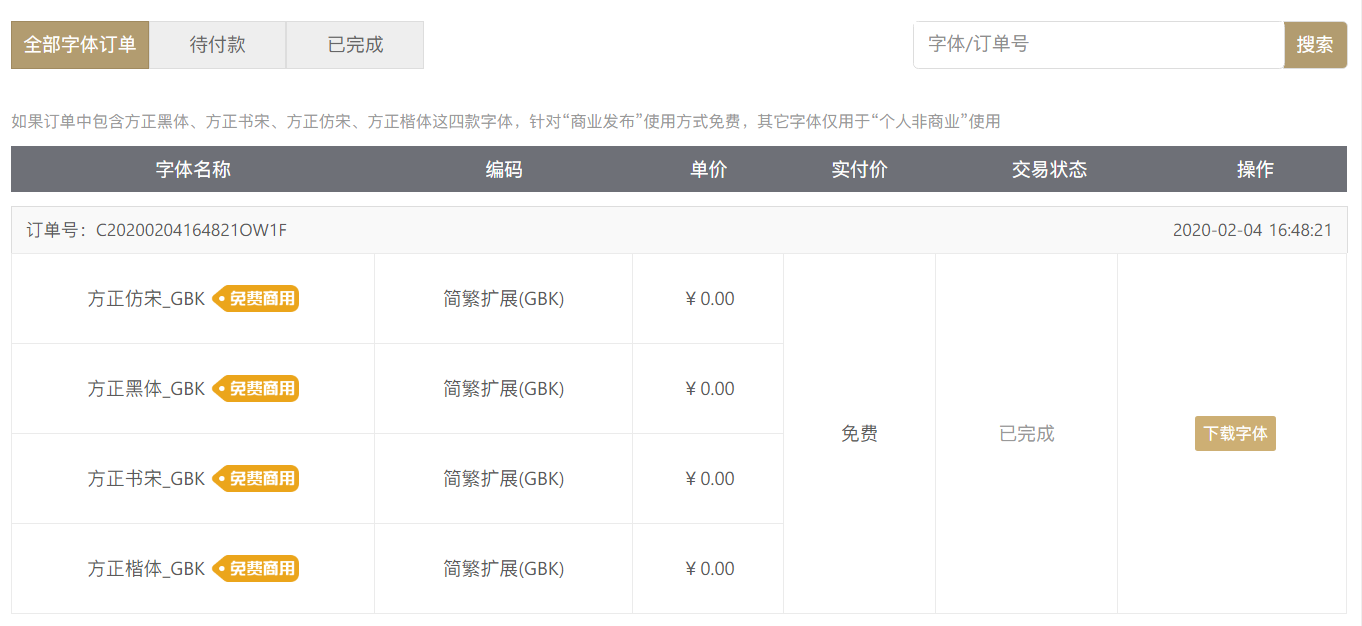
\includegraphics[width=0.9\textwidth]{founder.png}
\end{figure}

\subsection{其他中文字体}
如果你想完全自定义字体\footnote{这里仍然以方正字体为例。},你可以选择 \lstinline{chinesefont=nofont},然后在导言区设置
\begin{lstlisting}
\setCJKmainfont[BoldFont={FZHei-B01},ItalicFont={FZKai-Z03}]{FZShuSong-Z01}
\setCJKsansfont[BoldFont={FZHei-B01}]{FZKai-Z03}
\setCJKmonofont[BoldFont={FZHei-B01}]{FZFangSong-Z02}
\setCJKfamilyfont{zhsong}{FZShuSong-Z01}
\setCJKfamilyfont{zhhei}{FZHei-B01}
\setCJKfamilyfont{zhkai}[BoldFont={FZHei-B01}]{FZKai-Z03}
\setCJKfamilyfont{zhfs}[BoldFont={FZHei-B01}]{FZFangSong-Z02}
\newcommand*{\songti}{\CJKfamily{zhsong}}
\newcommand*{\heiti}{\CJKfamily{zhhei}}
\newcommand*{\kaishu}{\CJKfamily{zhkai}}
\newcommand*{\fangsong}{\CJKfamily{zhfs}}
\end{lstlisting}

\chapter{ElegantBook 写作示例}

\begin{introduction}
  \item 积分定义~\ref{def:int}
  \item Fubini 定理~\ref{thm:fubi}
  \item 最优性原理~\ref{pro:max}
  \item 柯西列性质~\ref{property:cauchy}
  \item 韦达定理
\end{introduction}

\section{Lebesgue 积分}
在前面各章做了必要的准备后,本章开始介绍新的积分。在 Lebesgue 测度理论的基础上建立了 Lebesgue 积分,其被积函数和积分域更一般,可以对有界函数和无界函数统一处理。正是由于 Lebesgue 积分的这些特点,使得 Lebesgue 积分比 Riemann 积分具有在更一般条件下的极限定理和累次积分交换积分顺序的定理,这使得 Lebesgue 积分不仅在理论上更完善,而且在计算上更灵活有效。

Lebesgue 积分有几种不同的定义方式。我们将采用逐步定义非负简单函数,非负可测函数和一般可测函数积分的方式。

由于现代数学的许多分支如概率论、泛函分析、调和分析等常常用到一般空间上的测度与积分理论,在本章最后一节将介绍一般的测度空间上的积分。

\subsection{积分的定义}

我们将通过三个步骤定义可测函数的积分。首先定义非负简单函数的积分。以下设 $E$ 是 $\mathcal{R}^n$ 中的可测集。

\begin{definition}[可积性] \label{def:int} 
设 $ f(x)=\sum\limits_{i=1}^{k} a_i \chi_{A_i}(x)$ 是 $E$ 上的\textbf{非负简单函数},中文其中 $\{A_1,A_2,\ldots,A_k\}$ 是 $E$ 上的一个可测分割,$a_1,a_2,\ldots,a_k$ 是非负实数。定义 $f$ 在 $E$ 上的积分为 $\int_{a}^b f(x)$
\begin{equation}
   \label{inter}
   \int_{E} f dx = \sum_{i=1}^k a_i m(A_i) \pi \alpha\beta\sigma\gamma\nu\xi\epsilon\varepsilon. \oint_{a}^b\ointop_{a}^b\prod_{i=1}^n
\end{equation}
一般情况下 $0 \leq \int_{E} f dx \leq \infty$。若 $\int_{E} f dx < \infty$,则称 $f$ 在 $E$ 上可积。
\end{definition}

一个自然的问题是,Lebesgue 积分与我们所熟悉的 Riemann 积分有什么联系和区别?在 4.4 在我们将详细讨论 Riemann 积分与 Lebesgue 积分的关系。这里只看一个简单的例子。设 $D(x)$ 是区间 $[0,1]$ 上的 Dirichlet 函数。即 $D(x)=\chi_{Q_0}(x)$,其中 $Q_0$ 表示 $[0,1]$ 中的有理数的全体。根据非负简单函数积分的定义,$D(x)$ 在 $[0,1]$ 上的 Lebesgue 积分为
\begin{equation}
   \label{inter2}
   \int_0^1 D(x)dx = \int_0^1 \chi_{Q_0} (x) dx = m(Q_0) = 0
\end{equation}
即 $D(x)$ 在 $[0,1]$ 上是 Lebesgue 可积的并且积分值为零。但 $D(x)$ 在 $[0,1]$ 上不是 Riemann 可积的。


有界变差函数是与单调函数有密切联系的一类函数。有界变差函数可以表示为两个单调递增函数之差。与单调函数一样,有界变差函数几乎处处可导。与单调函数不同,有界变差函数类对线性运算是封闭的,它们构成一线空间。练习题 \ref{exer:43} 是一个性质的证明。

\begin{exercise}\label{exer:43}
设 $f \notin\in L(\mathcal{R}^1)$,$g$ 是 $\mathcal{R}^1$ 上的有界可测函数。证明函数
\begin{equation}
   \label{ex:1}
   I(t) = \int_{\mathcal{R}^1} f(x+t)g(x)dx \quad t \in \mathcal{R}^1
\end{equation}
是 $\mathcal{R}^1$ 上的连续函数。 
\end{exercise}

\begin{solution}
即 $D(x)$ 在 $[0,1]$ 上是 Lebesgue 可积的并且积分值为零。但 $D(x)$ 在 $[0,1]$ 上不是 Riemann 可积的。
\end{solution}

\begin{proof}
即 $D(x)$ 在 $[0,1]$ 上是 Lebesgue 可积的并且积分值为零。但 $D(x)$ 在 $[0,1]$ 上不是 Riemann 可积的。
\end{proof}

\begin{theorem}[Fubini 定理] \label{thm:fubi} 
(1)若 $f(x,y)$ 是 $\mathcal{R}^p\times\mathcal{R}^q$ 上的非负可测函数,则对几乎处处的 $x\in \mathcal{R}^p$,$f(x,y)$ 作为 $y$ 的函数是 $\mathcal{R}^q$ 上的非负可测函数,$g(x)=\int_{\mathcal{R}^q}f(x,y) dy$ 是 $\mathcal{R}^p$ 上的非负可测函数。并且
\begin{equation}
   \label{eq:461}
   \int_{\mathcal{R}^p\times\mathcal{R}^q} f(x,y) dxdy=\int_{\mathcal{R}^p}\left(\int_{\mathcal{R}^q}f(x,y)dy\right)dx.
\end{equation}

(2)若 $f(x,y)$ 是 $\mathcal{R}^p\times\mathcal{R}^q$ 上的可积函数,则对几乎处处的 $x\in\mathcal{R}^p$,$f(x,y)$ 作为 $y$ 的函数是 $\mathcal{R}^q$ 上的可积函数,并且 $g(x)=\int_{\mathcal{R}^q}f(x,y) dy$ 是 $\mathcal{R}^p$ 上的可积函数。而且~\ref{eq:461} 成立。
\end{theorem}

\ref{thm:fubi}

\begin{note}
在本模板中,引理(lemma),推论(corollary)的样式和定理~\ref{thm:fubi} 的样式一致,包括颜色,仅仅只有计数器的设置不一样。
\end{note}

我们说一个实变或者复变量的实值或者复值函数是在区间上平方可积的,如果其绝对值的平方在该区间上的积分是有限的。所有在勒贝格积分意义下平方可积的可测函数构成一个希尔伯特空间,也就是所谓的 $L^2$ 空间,几乎处处相等的函数归为同一等价类。形式上,$L^2$ 是平方可积函数的空间和几乎处处为 0 的函数空间的商空间。

\begin{proposition}[最优性原理] \label{pro:max}
如果 $u^*$ 在 $[s,T]$ 上为最优解,则 $u^*$ 在 $[s, T]$ 任意子区间都是最优解,假设区间为 $[t_0, t_1]$ 的最优解为 $u^*$ ,则 $u(t_0)=u^{*}(t_0)$,即初始条件必须还是在 $u^*$ 上。
\end{proposition}

我们知道最小二乘法可以用来处理一组数据,可以从一组测定的数据中寻求变量之间的依赖关系,这种函数关系称为经验公式。本课题将介绍最小二乘法的精确定义及如何寻求点与点之间近似成线性关系时的经验公式。假定实验测得变量之间的 $n$ 个数据,则在平面上,可以得到 $n$ 个点,这种图形称为 “散点图”,从图中可以粗略看出这些点大致散落在某直线近旁, 我们认为其近似为一线性函数,下面介绍求解步骤。

\begin{figure}[htbp]
  \centering
  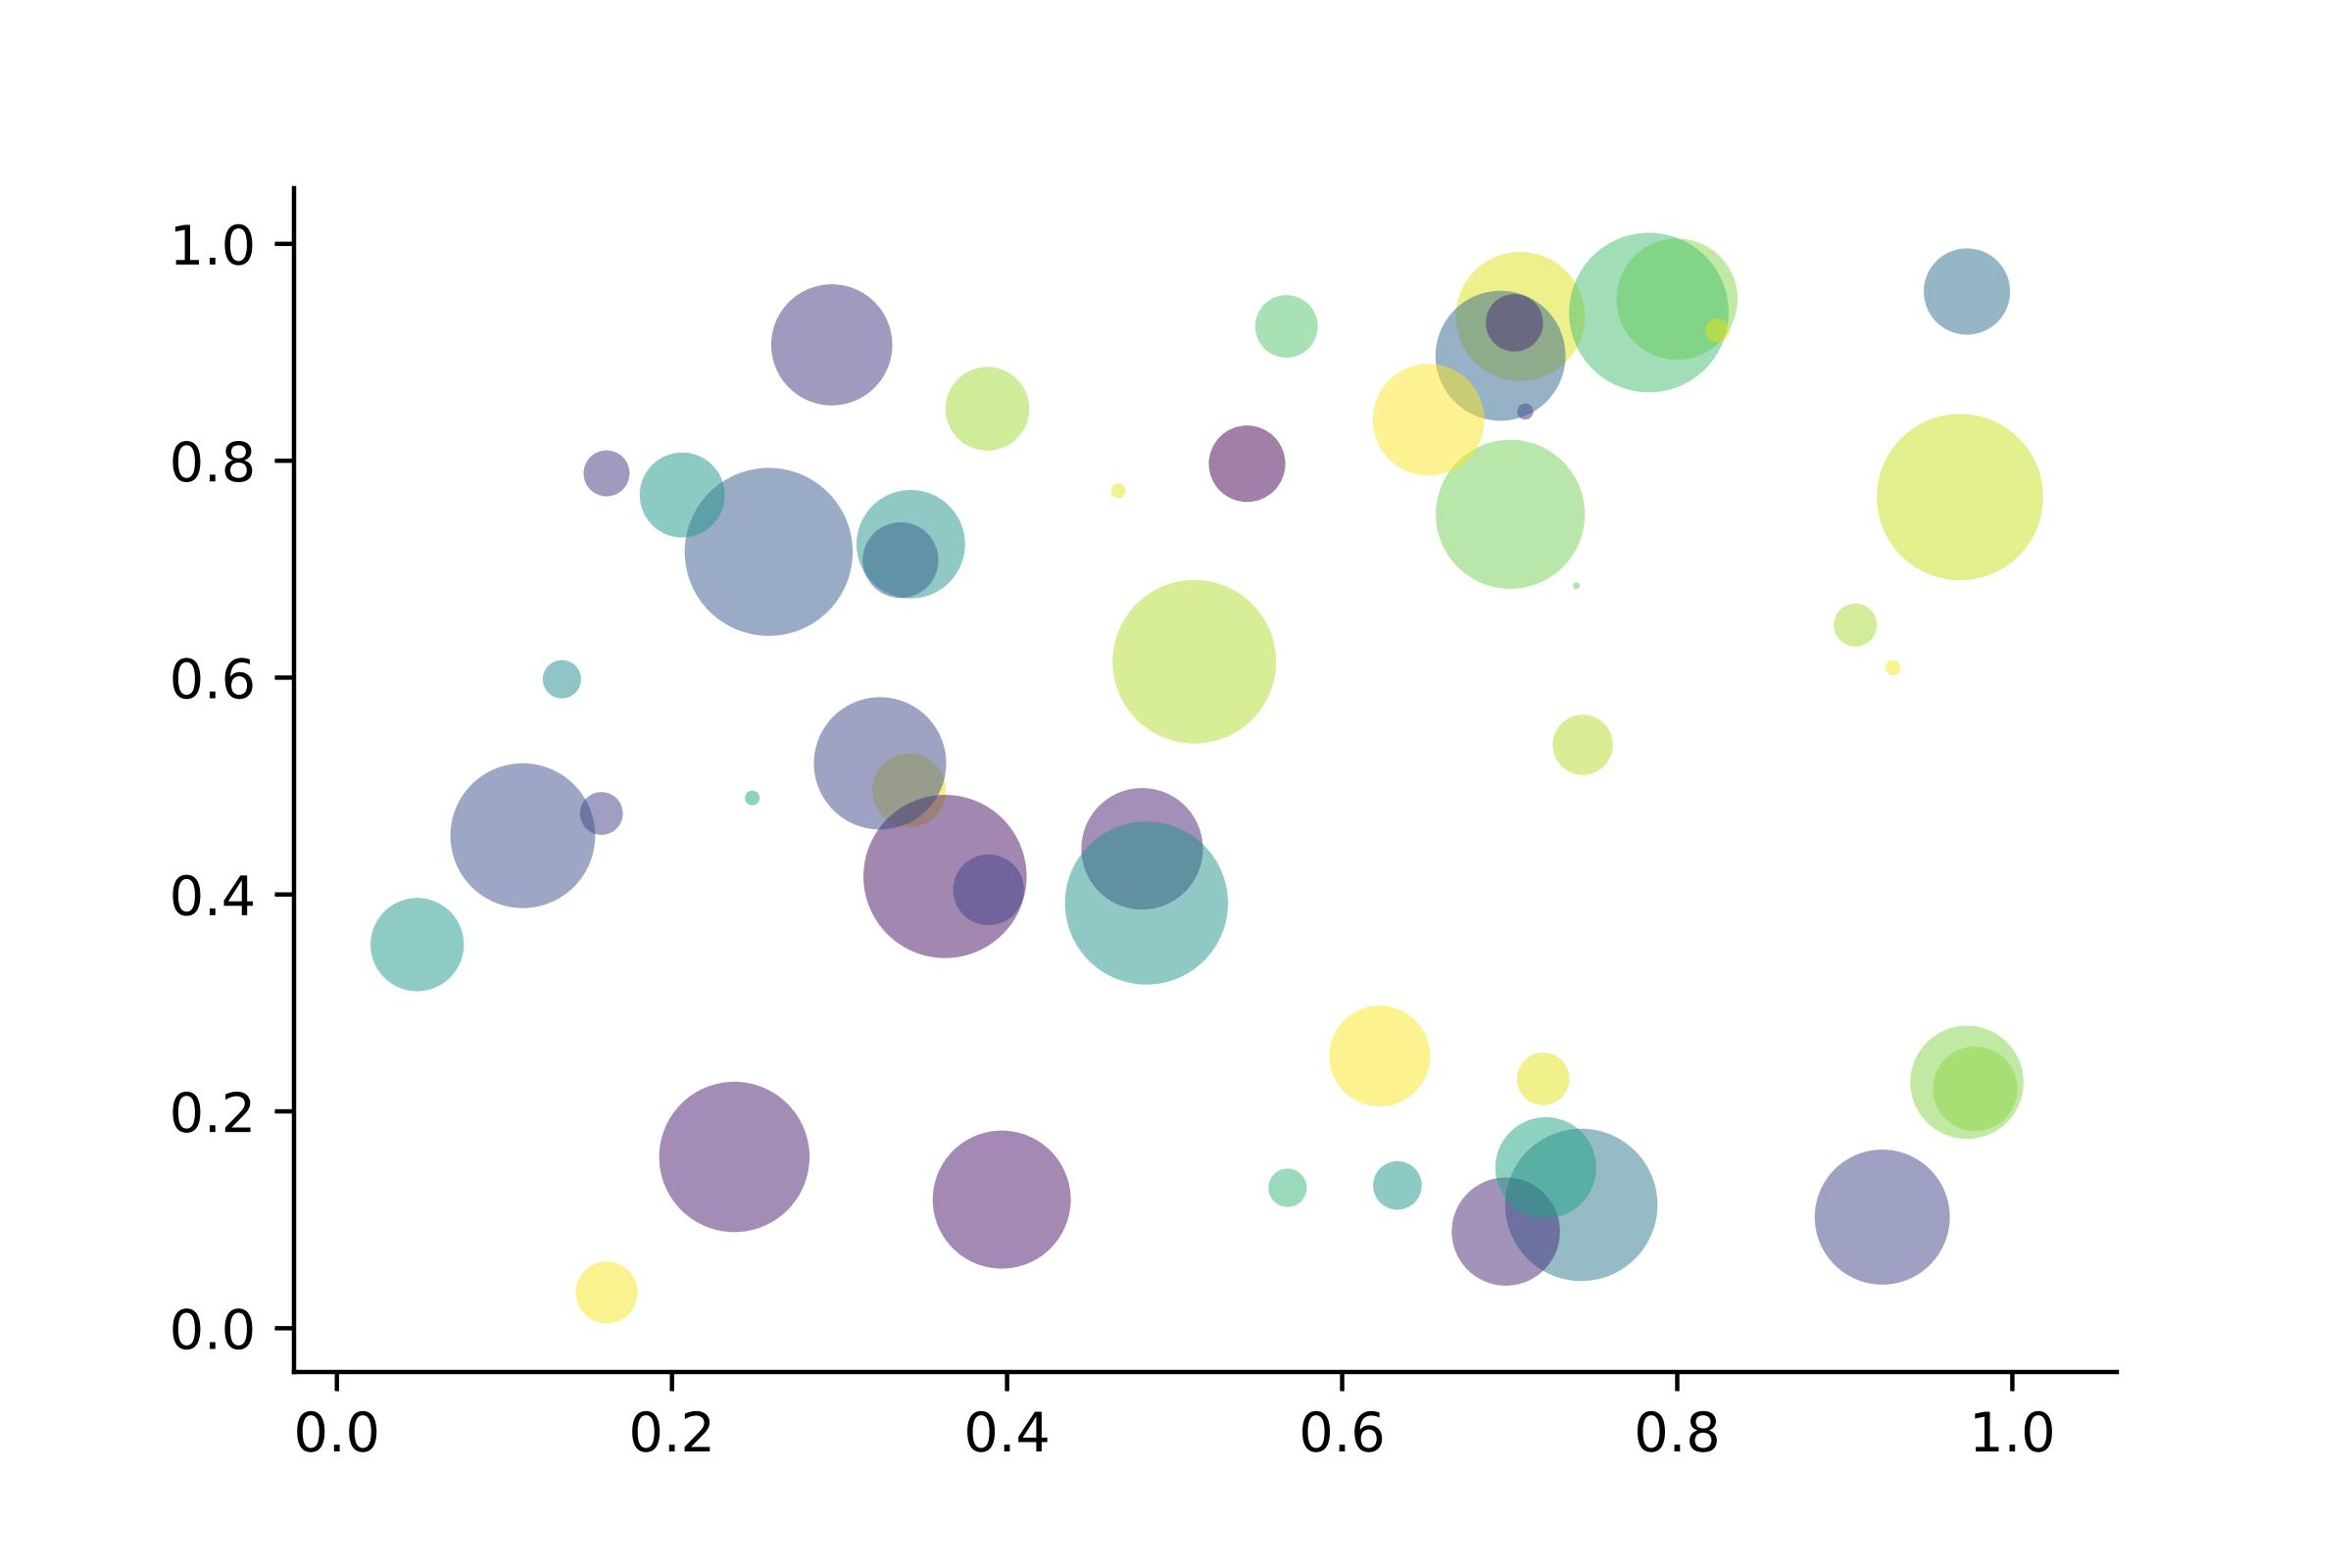
\includegraphics[width=0.6\textwidth]{scatter.jpg}
  \caption{散点图示例 $\hat{y}=a+bx$ \label{fig:scatter}}
\end{figure}

以最简单的一元线性模型来解释最小二乘法。什么是一元线性模型呢?监督学习中,如果预测的变量是离散的,我们称其为分类(如决策树,支持向量机等),如果预测的变量是连续的,我们称其为回归。回归分析中,如果只包括一个自变量和一个因变量,且二者的关系可用一条直线近似表示,这种回归分析称为一元线性回归分析。如果回归分析中包括两个或两个以上的自变量,且因变量和自变量之间是线性关系,则称为多元线性回归分析。对于二维空间线性是一条直线;对于三维空间线性是一个平面,对于多维空间线性是一个超平面。

\begin{property}\label{property:cauchy}
柯西列的性质
\begin{enumerate}
\item $\{x_k\}$ 是柯西列,则其子列 $\{x_k^i\}$ 也是柯西列。
\item $x_k\in \mathcal{R}^n$,$\rho(x,y)$ 是欧几里得空间,则柯西列收敛,$(\mathcal{R}^n,\rho)$ 空间是完备的。
\end{enumerate}
\end{property}

\begin{conclusion}
回归分析(regression analysis) 是确定两种或两种以上变量间相互依赖的定量关系的一种统计分析方法。运用十分广泛,回归分析按照涉及的变量的多少,分为一元回归和多元回归分析;按照因变量的多少,可分为简单回归分析和多重回归分析;按照自变量和因变量之间的关系类型,可分为线性回归分析和非线性回归分析。
\end{conclusion}

\begin{problemset}
\item 设 $A$ 为数域 $K$ 上的 $n$ 级矩阵。证明:如果 $K^n$ 中任意非零列向量都是 $A$ 的特征向量,则 $A$ 一定是数量矩阵。
\item 证明:不为零矩阵的幂零矩阵不能对角化。
\item 设 $A = (a_{ij})$ 是数域 $K$ 上的一个 $n$ 级上三角矩阵,证明:如果 $a_{11} = a_{22} = \cdots = a_{nn}$,并且至少有一个 $a_{kl} \not = 0 (k < l)$,则 $A$ 一定不能对角化。
\end{problemset}

\chapter{常见问题集}

我们根据用户社区反馈整理了下面一些常见的问题,用户在遇到问题时,应当首先查阅本手册和本部分的常见的问题。

\begin{enumerate}[itemsep=1.5ex]
  \item \question{有没有办法章节用“第一章,第一节,(一)”这种?}
    见前文介绍,可以使用 \lstinline{scheme=chinese} 设置。
  \item \question{大佬,我想把正文字体改为亮色,背景色改为黑灰色。}
    页面颜色可以使用 \lstinline{\pagecolor} 命令设置,文本命令可以参考\href{https://tex.stackexchange.com/questions/278544/xcolor-what-is-the-equivalent-of-default-text-color}{这里}进行设置。
  \item \question{\lstinline[breaklines]{Package ctex Error: CTeX fontset 'Mac' is unavailable.}}
    在 Mac 系统下,中文编译请使用 \hologo{XeLaTeX}。
  \item \question{\lstinline{! LaTeX Error: Unknown option 'scheme=plain' for package 'ctex'.}}
    你用的 C\TeX{} 套装吧?这个里面的 \lstinline{ctex} 宏包已经是已经是 10 年前的了,与本模板使用的 \lstinline{ctex} 宏集有很大区别。不建议 C\TeX{} 套装了,请卸载并安装 \TeX{} Live 2022。
  \item \question{我该使用什么版本?}
    请务必使用\href{https://github.com/ElegantLaTeX/ElegantBook/releases}{最新正式发行版},发行版间不定期可能会有更新(修复 bug 或者改进之类),如果你在使用过程中没有遇到问题,不需要每次更新\href{https://github.com/ElegantLaTeX/ElegantBook/archive/master.zip}{最新版},但是在发行版更新之后,请尽可能使用最新版(发行版)!最新发行版可以在 GitHub 或者 \TeX{} Live 2021 内获取。
  \item \question{我该使用什么编辑器?}
    你可以使用 \TeX{} Live 2021 自带的编辑器 \TeX{}works 或者使用 \TeX{}studio,\TeX works 的自动补全,你可以参考我们的总结 \href{https://github.com/EthanDeng/texworks-autocomplete}{\TeX works 自动补全}。推荐使用 \TeX{} Live 2021 + \TeX{}studio。我自己用 VS Code 和 Sublime Text,相关的配置说明,请参考 \href{https://github.com/EthanDeng/vscode-latex}{\LaTeX{} 编译环境配置:Visual Studio Code 配置简介} 和 \href{https://github.com/EthanDeng/sublime-text-latex}{Sublime Text 搭建 \LaTeX{} 编写环境}。
  \item \question{您好,我们想用您的 ElegantBook 模板写一本书。关于机器学习的教材,希望获得您的授权,谢谢您的宝贵时间。}
    模板的使用修改都是自由的,你们声明模板来源以及模板地址(GitHub 地址)即可,其他未尽事宜按照开源协议 LPPL-1.3c。做好之后,如果方便的话,可以给我们一个链接,我把你们的教材放在 Elegant\LaTeX{} 用户作品集里。
  \item \question{请问交叉引用是什么?}
    本群和本模板适合有一定 \LaTeX{} 基础的用户使用,新手请先学习 \LaTeX{} 的基础,理解各种概念,否则你将寸步难行。
  \item \question{代码高亮环境能用其他语言吗?}
    可以的,ElegantBook 模板用的是 \lstinline{listings} 宏包,你可以在环境(\lstinline{lstlisting})之后加上语言(比如 Python 使用 \lstinline{language=Python} 选项),全局语言修改请使用 \lstinline{lsset} 命令,更多信息请参考宏包文档。
  \item \question{群主,什么时候出 Beamer 的模板(主题),ElegantSlide 或者 ElegantBeamer?}
    由于 Beamer 中有一个很优秀的主题 \href{https://github.com/matze/mtheme}{Metropolis}。后续确定不会再出任何主题/模板,请大家根据需要修改已有主题。
\end{enumerate}

\chapter{版本更新历史}

根据用户的反馈,我们不断修正和完善模板。由于 3.00 之前版本与现在版本差异非常大,在此不列出 3.00 之前的更新内容。


\datechange{2022/04/09}{版本 4.3 正式发布。}

\begin{change}
  \item 放弃 newtx 系列宏包的设置,改用 TeX Gyre Terms,并设置其他字体;
  \item 修改定理类环境内部字体设置,修复环境内部中文无法加粗问题;
  \item 增加定理类环境的计数器选项 \lstinline{thmcnt},可选 \lstinline{chapter} 和 \lstinline{section};
  \item 增加 \lstinline{bibend} 选项,可选 \lstinline{bibend=biber}(默认)和 \lstinline{bibend=bibtex}。
\end{change}



\datechange{2022/03/08}{版本 4.2 正式发布。}

\begin{change}
  \item 对于 newtx 系列宏包更新导致的字体 bug 的修复;
  \item 修缮目录格式,为了达到这个目的,重新改写 \lstinline{\chaptername} 的重定义语句;
  \item 增加日语 \lstinline{lang=jp} 设定。
  \item 这个版本为一个临时性版本,在 \TeX Live 2022 发布之后,将尽快发布 4.3 版本,由于对于中文的改动比较大,可能会出现预期之外的 bug,有问题可以在 QQ 群或者 Github 反馈。
\end{change}


\datechange{2021/05/02}{版本 4.1 正式发布。}

\begin{change}
  \item \textbf{重要改动}:由原先的 \hologo{BibTeX} 改为 biblatex 编译方式(后端为 \lstinline{biber}),请注意两者之间的差异;
  \item \textbf{重要改进}:修改对于定理写法兼容方式,提高数学公式代码的兼容性;
  \item 页面设置改动,默认页面更宽;方便书写和阅读;
  \item 支持目录文字以及页码跳转;
  \item 不再维护 \hologo{pdfLaTeX} 中文支持方式,请务必使用 \hologo{XeLaTeX} 编译中文文稿。
  \item 增加多个语言选项,法语 \lstinline{lang=fr}、荷兰语 \lstinline{lang=nl}、匈牙利语 \lstinline{lang=hu}、西班牙语 \lstinline{lang=es}、蒙古语 \lstinline{lang=mn} 等。
\end{change}


\datechange{2020/04/12}{版本 3.11 正式发布,\textcolor{red}{此版本为 3.x 最后版本。}}

\begin{change}
  \item \textbf{重要修正}:修复因为 \lstinline{gbt7714} 宏包更新导致的 \lstinline{natbib option clash} 错误;
  \item 由于 \lstinline{pgfornament} 宏包未被 \TeX{} Live 2020 收录,因此删除 base 相关的内容;
  \item 修复部分环境的空格问题;
  \item 增加了意大利语言选项 \lstinline{lang=it}。
\end{change}


\datechange{2020/02/10}{版本 3.10 正式发布}

\begin{change}
  \item 增加数学字体选项 \lstinline{math},可选项为 \lstinline{newtx} 和 \lstinline{cm}。\\
  \textbf{重要提示}:原先通过 \lstinline{newtxmath} 宏包设置的数学字体改为 \LaTeX{} 默认数学字体,如果需要保持原来的字体,需要显式声明数学字体(\lstinline{math=newtx});
  \item 新增中文字体选项 \lstinline{chinesefont},可选项为 \lstinline{ctexfont}、\lstinline{founder} 和 \lstinline{nofont}。
  \item 将封面作者信息设置为可选,并且增加自定义信息命令 \lstinline{\bioinfo};
  \item 在说明文档中增加版本历史,新增 \lstinline{\datechange} 命令和 \lstinline{change} 环境;
  \item 增加汉化章节选项 \lstinline{scheme},可选项为汉化 \lstinline{chinese};
  \item 由于 \lstinline{\lvert} 问题已经修复,重新调整 \lstinline{ctex} 宏包和 \lstinline{amsmath} 宏包位置。
  \item 修改页眉设置,去除了 \lstinline{\lastpage} 以避免 page anchor 问题,加入 \lstinline{\frontmatter}。
  \item 修改参考文献选项 \lstinline{cite},可选项为数字 \lstinline{numbers}、 作者-年份 \lstinline{authoryear} 以及上标 \lstinline{super}。
  \item 新增参考文献样式选项 \lstinline{bibstyle},并将英文模式下参考文献样式 \lstinline{apalike} 设置为默认值,中文仍然使用 \lstinline{gbt7714} 宏包设置。
\end{change}

\datechange{2019/08/18}{版本 3.09 正式发布}

\begin{change}
  \item \lstinline{\elegantpar} 存在 bug,删除 \lstinline{\elegantpar} 命令,建议用户改用 \lstinline{\marginnote} 和 \lstinline{\marginpar} 旁注命令。
  \item 积分操作符统一更改为 \lstinline{esint} 宏包设置;
  \item 新增目录选项 \lstinline{toc},可选项为单栏 \lstinline{onecol} 和双栏 \lstinline{twocol};
  \item 手动增加参考文献选项 \lstinline{cite},可选项为上标形式 \lstinline{super};
  \item 修正章节习题(\lstinline{problemset})环境。
\end{change}

\datechange{2019/05/28}{版本 3.08 正式发布}

\begin{change}
  \item 修复 \lstinline{\part} 命令。
  \item 引入 Note 模板中的 \lstinline{pad} 选项 \lstinline{device=pad}。
  \item 数学字体加入 \lstinline{mtpro2} 可选项 \lstinline{math=mtpro2},使用免费的 \lstinline{lite} 子集。
  \item 将参考文献默认显示方式 \lstinline{authoyear} 改为 \lstinline{numbers}。
  \item 引入旁注命令 \lstinline{\marginpar}(测试)。
  \item 新增章节摘要环境 \lstinline{introduction}。
  \item 新增章节习题环境 \lstinline{problemset}。
  \item 将 \lstinline{\equote} 重命名为 \lstinline{\extrainfo}。
  \item 完善说明文档,增加致谢部分。
\end{change}

\datechange{2019/04/15}{版本 3.07 正式发布}

\begin{change}
  \item 删除中英文自定义字体总设置。
  \item 新增颜色主题,并将原绿色默认主题设置为蓝色 \lstinline{color=blue}。
  \item 引入隐藏装饰图案选项 \lstinline{base},可选项有显示 \lstinline{show} 和隐藏 \lstinline{hide}。
  \item 新增定理模式 \lstinline{mode},可选项有简单模式 \lstinline{simple} 和炫彩模式 \lstinline{fancy}。
  \item 新增隐藏证明、答案等环境的选项 \lstinline{result=noanswer}。
\end{change}

\datechange{2019/02/25}{版本 3.06 正式发布}

\begin{change}
  \item 删除水印。
  \item 新封面,新装饰图案。
  \item 添加引言使用说明。
  \item 修复双面 \lstinline{twoside}。
  \item 美化列表环境。
  \item 增加 \lstinline{\subsubsection} 的设置。
  \item 将模板拆分成中英文语言模式。
  \item 使用 \lstinline{lstlisting} 添加代码高亮。
  \item 增加定理类环境使用说明。
\end{change}

\datechange{2019/01/22}{版本 3.05 正式发布}

\begin{change}
  \item 添加 \lstinline{xeCJK} 宏包中文支持方案。
  \item 修复模板之前对 Ti\textit{k}Z 单位的改动。
  \item 更新 logo 图。
\end{change}

\datechange{2019/01/15}{版本 3.04 正式发布}

\begin{change}
  \item 格式化模板代码。
  \item 增加 \lstinline{\equote} 命令。
  \item 修改 \lstinline{\date}。
\end{change}

\datechange{2019/01/08}{版本 3.03 正式发布}

\begin{change}
  \item 修复附录章节显示问题。
  \item 小幅优化封面代码。
\end{change}

\datechange{2018/12/31}{版本 3.02 正式发布}

\begin{change}
  \item 修复名字系列命令自定义格式时出现的空格问题,比如 \lstinline{\listfigurename}。
  \item 英文定理类名字改为中文名。
  \item 英文结构名改为中文。
\end{change}

\datechange{2018/12/16}{版本 3.01 正式发布}

\begin{change}
  \item 调整 \lstinline{ctex} 宏包。
  \item 说明文档增加更新内容。
\end{change}

\datechange{2018/12/06}{版本 3.00 正式发布}

\begin{change}
  \item 删除 \lstinline{mathpazo} 数学字体选项。
  \item 添加邮箱命令 \lstinline{\mailto}。
  \item 修改英文字体为 \lstinline{newtx} 系列,另外大型操作符号维持 cm 字体。
  \item 中文字体改用 \lstinline{ctex} 宏包自动设置。
  \item 删除 \lstinline{xeCJK} 字体设置,原因是不同系统字体不方便统一。
  \item 定理换用 \lstinline{tcolobox} 宏包定义,并基本维持原有的定理样式,优化显示效果,支持跨页;定理类名字重命名,如 etheorem 改为 theorem 等等。
  \item 删去自定义的缩进命令 \lstinline{\Eindent}。
  \item 添加参考文献宏包 \lstinline{natbib}。
  \item 颜色名字重命名。
\end{change}

\nocite{*}
\printbibliography[heading=bibintoc, title=\ebibname]
\appendix

\chapter{基本数学工具}


本附录包括了计量经济学中用到的一些基本数学,我们扼要论述了求和算子的各种性质,研究了线性和某些非线性方程的性质,并复习了比例和百分数。我们还介绍了一些在应用计量经济学中常见的特殊函数,包括二次函数和自然对数,前 4 节只要求基本的代数技巧,第 5 节则对微分学进行了简要回顾;虽然要理解本书的大部分内容,微积分并非必需,但在一些章末附录和第 3 篇某些高深专题中,我们还是用到了微积分。

\section{求和算子与描述统计量}

\textbf{求和算子} 是用以表达多个数求和运算的一个缩略符号,它在统计学和计量经济学分析中扮演着重要作用。如果 $\{x_i: i=1, 2, \ldots, n\}$ 表示 $n$ 个数的一个序列,那么我们就把这 $n$ 个数的和写为:

\begin{equation}
\sum_{i=1}^n x_i \equiv x_1 + x_2 +\cdots + x_n
\end{equation}



\end{document}
